\section{Object Tracking}
\begin{frame}{}
    \LARGE Image Segmentation: \textbf{Object Tracking}
\end{frame}

\begin{frame}{Goal of Object Tracking}
    \begin{itemize}
        \item Track objects over a sequence of photos or a video
        \item Exceedingly challenging in multi-object tracking scenarios
        \item Need to ensure objects are not mixed up or lost midway
    \end{itemize}
\end{frame}

\begin{frame}[allowframebreaks]{A Common Solution}
    \begin{itemize}
        \item Perform object detection in each frame
        \item Assign unique IDs to each detected object
        \item Store feature vectors for each object (e.g., appearance, position)
        \item Track objects across frames based on their IDs and feature vectors
    \end{itemize}
\framebreak
    \begin{figure}
        \centering
        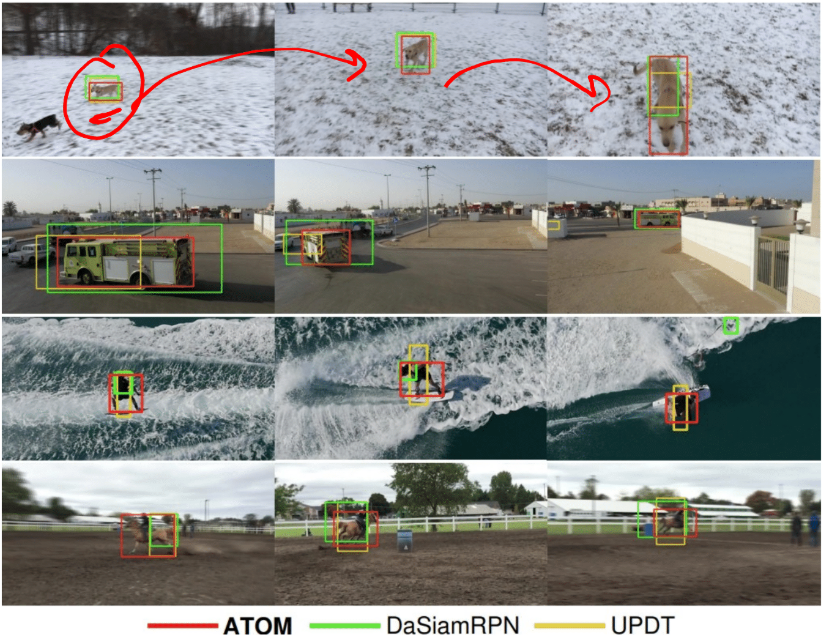
\includegraphics[width=1.0\textwidth,height=0.8\textheight,keepaspectratio]{images/segmentation/obj-tracking.png}
        \caption*{Comparison of 3 approaches for Object Tracking}
    \end{figure}
\end{frame}